\documentclass[11pt,t]{beamer}
%% Language and font encodings
\usepackage[english]{babel}
\usepackage[utf8x]{inputenc}
\usepackage[T1]{fontenc}

\usepackage{helvet}

%% Sets page size and margins
\usepackage[letterpaper,top=3cm,bottom=2cm,left=3cm,right=3cm,marginparwidth=1.75cm]{geometry}

%% Useful packages
\usepackage{amsmath}
\usepackage{graphicx}
\usepackage{tcolorbox}
\usepackage{amssymb}
\usepackage{amsthm}
\usepackage{lastpage}
\usepackage{accents}
\usepackage{multicol}

% For better list numbering
\usepackage[shortlabels]{enumitem}

% Font
% \usepackage{tgbonum}


% Tikz
\usepackage{tikz}

\usetikzlibrary{calc,fit,shapes.misc,backgrounds}
\usepackage{pgfplots}
\pgfplotsset{compat = newest}
\usetikzlibrary{positioning, arrows.meta}
\usepgfplotslibrary{fillbetween}

% Headers
\usepackage{fancyhdr}
\pagestyle{fancy}

% Store \@title as \thetitle
\makeatletter
\let\thetitle\@title
\makeatother

\fancyhf{}
\lhead{\fontfamily{qbk}\fontsize{10}{11}\selectfont ECON 3070}
\rhead{\fontfamily{qbk}\fontsize{10}{11}\selectfont \thetitle}
\rfoot{\fontfamily{qbk}\fontsize{10}{11}\selectfont \thepage}


% Sections and Subsections

% define colors
\definecolor{buff-gold}{HTML}{CFB87C}
\definecolor{buff-grey}{HTML}{565A5C}
% custom tcolorbox
\tcbset{colframe=buff-gold, colback=white!100!black}

% new page per section
\usepackage{titlesec}
\newcommand{\sectionbreak}{\clearpage}
% change style of section
\usepackage{sectsty}
\sectionfont{\color{buff-gold} \fontfamily{qbk}\selectfont}
\subsectionfont{\color{buff-grey} \fontfamily{qbk}\selectfont}


\author{Kyle Butts}
\title{Lecture 8 - Cost Curves}
\subtitle{ECON 3070 - Intermediate Microeconomic Theory}

\begin{document}

\begin{frame}
  \titlepage
\end{frame}

\begin{frame}{Overview}
  In the previous lecture, we began talking about costs.

  \begin{itemize}
    \item We considered how output varies as we change the level of inputs (production function).
    
    \item And how firms choose the mix of inputs that produces a given quantity at the lowest price (optimal production).
    
    \item We considered what happens to the firm's lowest-cost input combination when prices or quantity changed (comparative statics).
    
    \item And we looked at how a firm chooses their input combination when the quantity of some input is fixed (short-run production).
  \end{itemize}
\end{frame}

\begin{frame}{Overview}
  In this section, we will learn how to calculate total, marginal, and average costs, both in the short run and the long run.

  \begin{itemize}
    \item We will look at these costs graphically, and analyze their relationship.
    \item We will also introduce concepts such as economies of scale, scope, and experience.
  \end{itemize}

\end{frame}

\begin{frame}{Long Run Total Cost Curve}
  In the previous chapter, we learned how to calculate total costs as a function of $Q$, $w$, and $r$.
  
  \bigskip\pause
  Remember that 
  $$
  TC = w*L^*(w,r,Q)+r*K^*(w,r,Q)
  $$
  where $L$ and $K$ are the cost-minimizing levels of labor and capital.

  \begin{itemize}
    \item Optimal $L$ and $K$ are functions of the wage, the rental rate, and the output quantity.
  \end{itemize}
  
\end{frame}

\begin{frame}{Long Run Total Cost Curve}
  \begin{figure}
    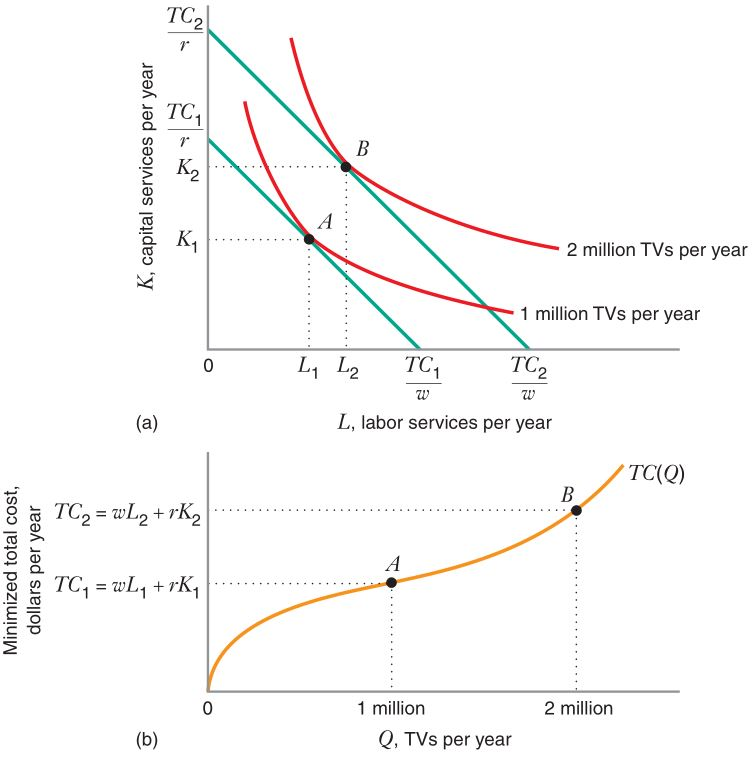
\includegraphics[width=200px]{figures/fig8_1.jpg}
  \end{figure}
\end{frame}

\begin{frame}{Long Run Total Cost Curve}
  Note that the total cost curve is always upward sloping.

  \begin{itemize}
    \item Suppose you could produce 100 units for \$1,000, and 150 units for \$900.
    \item Then you could also produce 100 units  for \$900 ... by producing 150, and throwing some away!
  \end{itemize}

  \bigskip \pause
  Also note that in the long run, $Q(0)=0$.

 \begin{itemize}
  \item Since all inputs can vary, the cost-minimizing level of all inputs needed to produce 0 units of output is \$0.
 \end{itemize}
\end{frame}

\begin{frame}\bgCoral{Try It Yourself}

\bigskip
Suppose a firm has the total cost function $TC(Q)=\frac{Q}{25}\sqrt{wr}$. Is the total cost curve increasing with $Q$? Do costs increase for the firm when the cost of capital $r$ increases?
\end{frame}

\begin{frame}{Comparative Statics of Long-run Total Cost}
  When the price of one input increases, the firm may substitute away from that input, but their TC still increases.

  \begin{itemize}
    \item If TC stayed the same at the higher input price, why wouldn't they have chosen that input combination to start with?

    \item And in most cases, the increase in cost is greater when a larger quantity is being produced.
  \end{itemize}

\end{frame}

\begin{frame}{Comparative Statics of LRTC}
  \begin{figure}
    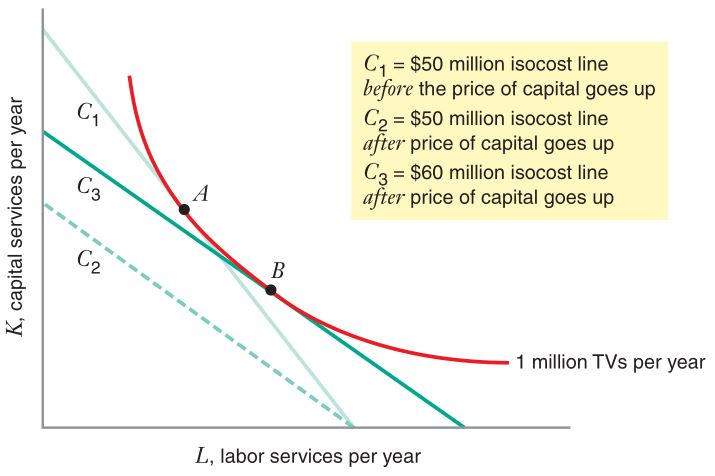
\includegraphics[width=260px]{figures/fig8_3.jpg}
  \end{figure}
\end{frame}

\begin{frame}{Comparative Statics of LRTC}
  \begin{figure}
    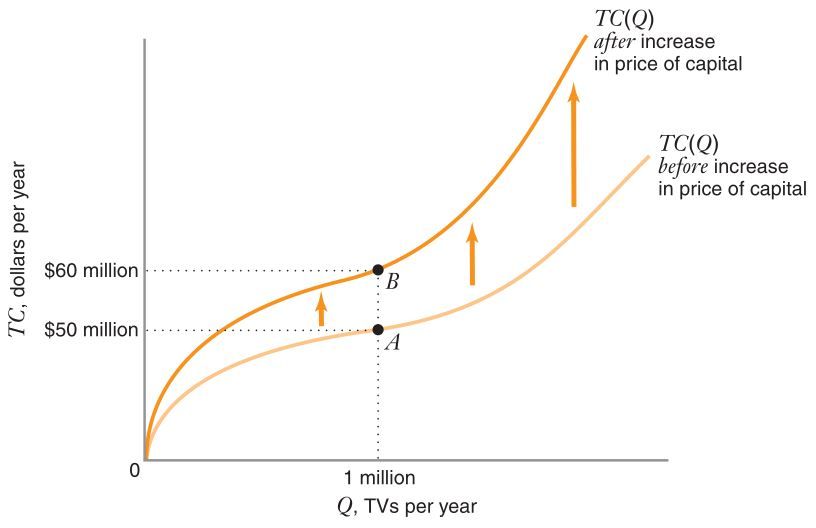
\includegraphics[width=260px]{figures/fig8_4.jpg}
  \end{figure}
\end{frame}

\begin{frame}{Comparative Statics of LRTC}
  What if both input prices increase proportionally?

  \bigskip\pause
  Then the slope of the isoquants $(-w/r)$ doesn't change.

  \begin{itemize}
    \item So the point of tangency doesn't change.
    
    \item In other words, the optimality condition still holds.
  \end{itemize}

  \bigskip\pause
  $\implies$ The input combination doesn't change. It just gets proportionally more expensive to make.
\end{frame}

\begin{frame}{Comparative Statics of LRTC}
  \begin{figure}
    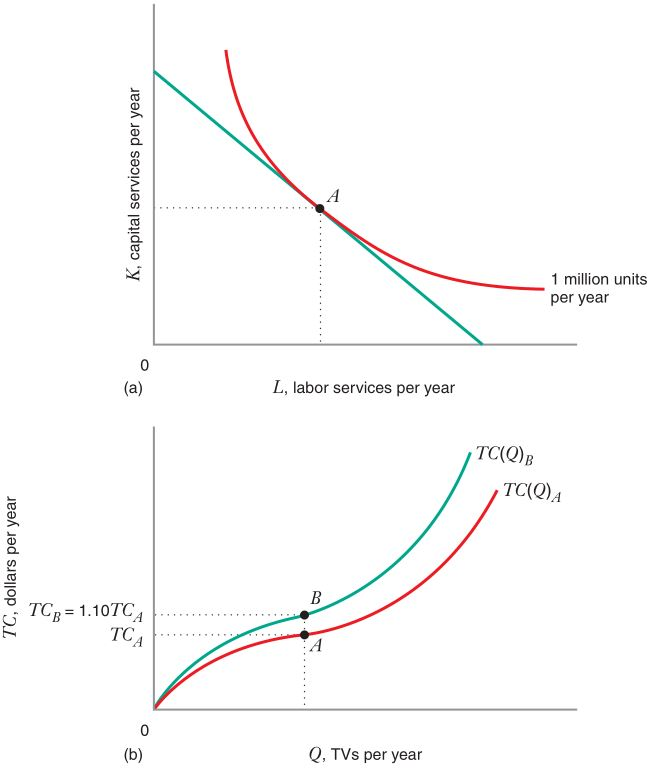
\includegraphics[width=180px]{figures/fig8_5.jpg}
  \end{figure}
\end{frame}

\begin{frame}{Long-Run Average and Marginal Costs}
  There are two other important costs we need to consider: \emph{marginal cost} and \emph{average cost}.

  \begin{itemize}
    \item Marginal cost is important in deciding \emph{how many} units to produce.
    
    \smallskip\textbf{How much should the firm produce?}
    
    \bigskip
    \item Average cost is useful in determining a firm's overall profitability (should they produce anything at all).
    
    \smallskip\textbf{Should they be producing at all?}
  \end{itemize}
\end{frame}

\begin{frame}{Long-Run Average and Marginal Costs}
  \textbf{Long-run average cost} is the firm's cost per unit of output.

  $$AC(Q) = \frac{TC(Q)}{Q}$$

  Also the slope of a ray from the origin to the point on the total cost curve.


  \bigskip
  \textbf{Long-run marginal cost} is the rate at which long-run total cost changes with respect to a change in output.

  $$MC(Q) = \frac{\Delta TC}{\Delta Q}$$

  Also the slope of the tangent line at that quantity.
\end{frame}

\begin{frame}{Long-Run Average and Marginal Costs}
  \begin{figure}
    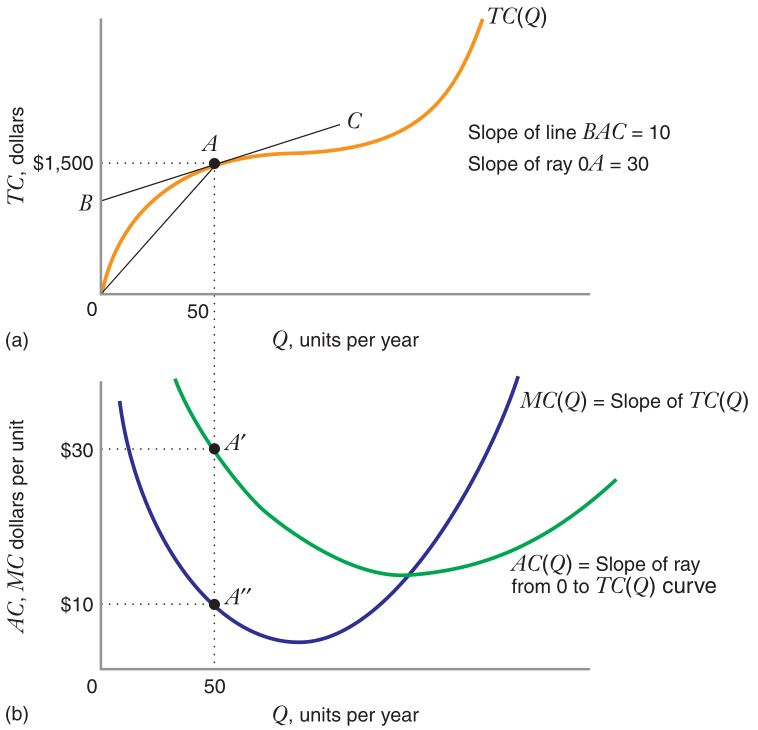
\includegraphics[width=200px]{figures/fig8_7.jpg}
  \end{figure}
\end{frame}

\begin{frame}{\bgCoral{Try It Yourself}}
  \bigskip
  Suppose that at the total cost function for a cost-minimizing firm is given by $TC(Q) = 4Q$. What is the firm's marginal and total cost?
\end{frame}

\begin{frame}{Relationship Between AC and MC Curves}
  As we saw with marginal product and average product, there is a systematic relationship between marginal cost and average cost.

  \begin{itemize}
    \item If average cost is decreasing as quantity is increasing, then average cost is greater than marginal cost.

    \item If average cost is increasing as quantity is increasing, then average cost is less than marginal cost.

    \item If average cost is constant as quantity is increasing, then average cost equals marginal cost.
  \end{itemize}
\end{frame}

\begin{frame}{Relationship Between AC and MC Curves}
  \begin{figure}
    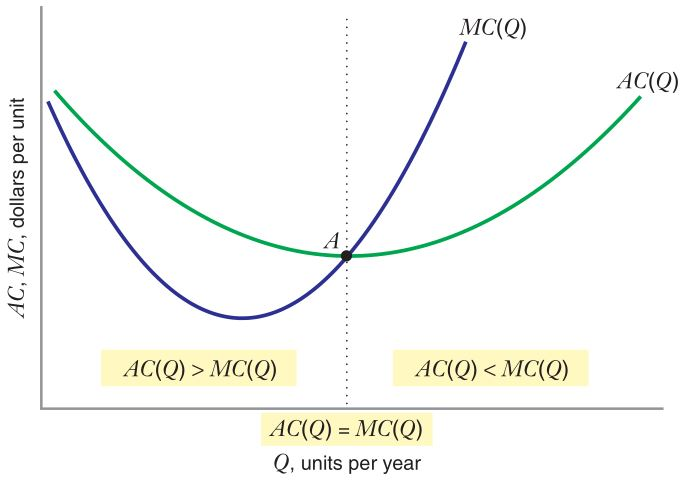
\includegraphics[width=240px]{figures/fig8_9.jpg}
  \end{figure}
\end{frame}

\begin{frame}{Economies of Scale}
  It's important to consider what will happen to a firm's production costs as they produce more output.

  \begin{itemize}
    \item Perhaps aas a firm produces more output, employees can specialize more...
    
    \item ... or maybe their production process uses \emph{indivisible inputs}, which cannot be scaled down easily...
    
    \item ...and their cost per unit falls.
  \end{itemize}
  
  \bigskip
  A firm is said to experience \textbf{economies of scale} when average cost of production falls as output rises.
\end{frame}

\begin{frame}{Economies of Scale}
  Or perhaps as a firm grows, managerial needs outpace output growth increase the per-unit cost.

  \bigskip
  \begin{itemize}
    \item When costs arise due to an increase in managerial needs, this is known as \textbf{managerial diseconomies}.
    
    \item When average cost rises as output rises, a firm is said to experience \textbf{diseconomies of scale}.
  \end{itemize}
\end{frame}

\begin{frame}{Economies of Scale}
  A firm is said to be producing at it's \textbf{minimum efficient scale (MES)} when long-run average cost is at it's minimum.

  \begin{itemize}
    \item This is an important concept since it tells us, \emph{at best}, how efficiently firms can produce the good
  \end{itemize}


  \bigskip\pause
  Firms with a large minimum efficient scale relative to market size have greater economies of scale.
    
  \begin{itemize}
    \item In these markets, it is more difficult for smaller firms to compete.
  \end{itemize}
\end{frame}

\begin{frame}{Economies of Scale}
  \begin{figure}
    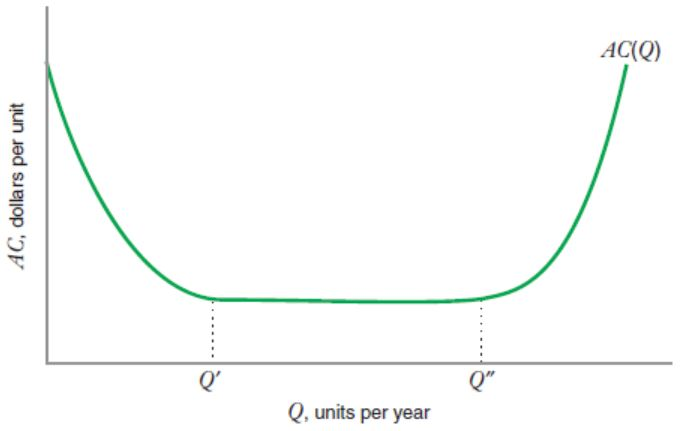
\includegraphics[width=260px]{figures/fig8_11.jpg}
  \end{figure}
\end{frame}

\begin{frame}{Economies of Scale and Returns to Scale}
  If average cost \textit{decreases} as output \textit{increases}, then we have \textit{economies of scale} and \textit{increasing returns to scale}.

  \begin{itemize}
    \item E.g. $Q=L^2$
  \end{itemize}

  \bigskip\pause
  If average cost \textit{increases} as output \textit{increases}, then we have \textit{diseconomies of scale} and \textit{decreasing returns to scale}.

  \begin{itemize}
    \item E.g. $Q=\sqrt{L}$
  \end{itemize}

  \bigskip\pause
  If average cost \textit{stays the same} as output \textit{increases}, then we have\textit{ neither economies nor diseconomies of scale} and \textit{constant returns to scale}.

  \begin{itemize}
    \item E.g. $Q=L$
  \end{itemize}
\end{frame}

\begin{frame}{Economies of Scale and Returns to Scale}
  
  Note that the previous slide assumed that input price didn't depend on quantity of production.

  \bigskip
  A firm could experience constant returns to scale in technology...

  \begin{itemize}
    \item ...but if quantity discounts are available for inputs, they may experience economies of scale.
    
    \pause
    \item Or if an input is scarce, the price may rise as output increases and that same firm may experience diseconomies of scale.
  \end{itemize}
\end{frame}

\begin{frame}{Measuring Economies of Scale}
  Can use elasticities to tell us how sensitive total cost is to output.

  The \textbf{output elasticity of total cost} is given by:

  $$
    \epsilon_{TC,Q}=\frac{\frac{\Delta TC}{TC}}{\frac{\Delta Q}{Q}}=\frac{\frac{\Delta TC}{\Delta Q}}{\frac{TC}{Q}}=\frac{MC}{AC}
  $$

  \bigskip
  \begin{figure}
    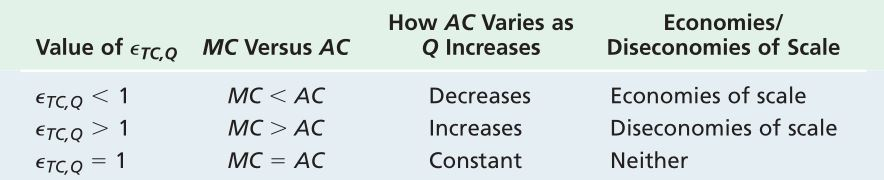
\includegraphics[width=280px]{figures/table8_3.jpg}
  \end{figure}
\end{frame}

\begin{frame}{\bgCoral{Try It Yourself}}

  Which of the following is a possible reason why a firm might experience increasing returns to scale, and diseconomies of scale?

  \begin{enumerate}[A)]
    \item The firm uses indivisible inputs in it's production process.
    \item The firm experiences managerial diseconomies when output rises.
    \item The firm receives quantity discounts on it's inputs when output rises.
    \item The firm's employees are able to specialize more when output rises.
  \end{enumerate}
\end{frame}

\begin{frame}{Short-Run Cost Curves}
  In the previous lecture, we learned the difference between the short run and the long run.

  \begin{itemize}
    \item In the short run, the levels some inputs cannot be varied.
    
    \item In the long run, the levels of \textit{all} inputs can.
    
    \item In this section, we will assume that capital (K) is the fixed input.
  \end{itemize}
\end{frame}

\begin{frame}{Short-Run Cost Curves}
  The short-run total cost curve $STC(Q)$ tells us the minimized total cost of producing $Q$ units of output when at least one input is fixed.

  \pause\bigskip
  The total cost curve can be divided into a \textbf{total variable cost curve (TVC)} and a \textbf{total fixed cost curve (TFC)}.

  \begin{itemize}
    \item $TVC(Q)$ is the sum of expenditures on variable inputs at the cost-minimizing input combination.
    
    \item $TFC(Q)$ is the total cost of fixed inputs.
  \end{itemize}

  $$
    STC(Q) = TVC(Q) + TFC(Q)
  $$

\end{frame}

\begin{frame}{Short-Run Cost Curves}
  Because we let capital be our fixed input, $TFC$ is simply the amount of money spent on $\bar{K}$ units of capital. In other words, $TFC = r\bar{K}$.

  \bigskip
  Thus, $STC(Q) = TVC(Q) + r\bar{K}$.
\end{frame}

\begin{frame}{Short-Run Cost Curves}
  Note that the vertical distance between the $STC(Q)$ curve and the $TVC(Q)$ curve is equal to $r\bar{K}$.

  \begin{figure}
    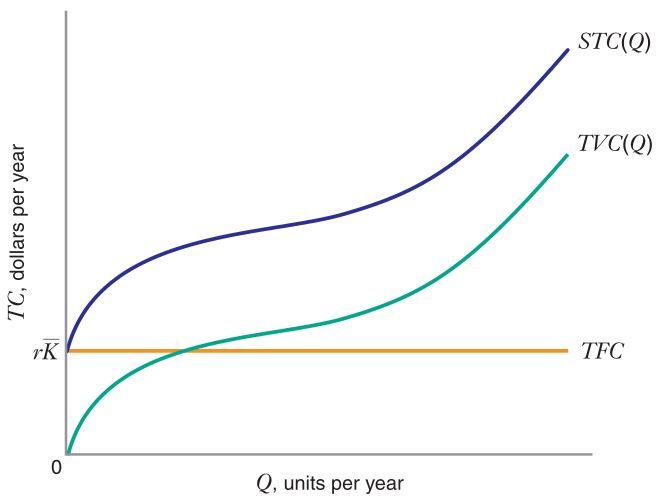
\includegraphics[width=210px]{figures/fig8_13.jpg}
  \end{figure}
\end{frame}

\begin{frame}{Relationship Between $LTC$ and $STC$}
  Consider a firm that produces televisions, and wants to expand production.

  \begin{itemize}
    \item In the short run, they can only adjust their level of labor.
    
    \item But in the long run, they can adjust the level of capital as well.
  \end{itemize}
\end{frame}

\begin{frame}{Relationship Between $LTC$ and $STC$}
  Going from $1$ million to $2$ million TVs. In the short run, you have to go to $B$. \only<2>{In the long run, you can go to $C$ at a lower cost.}
  \begin{figure}
    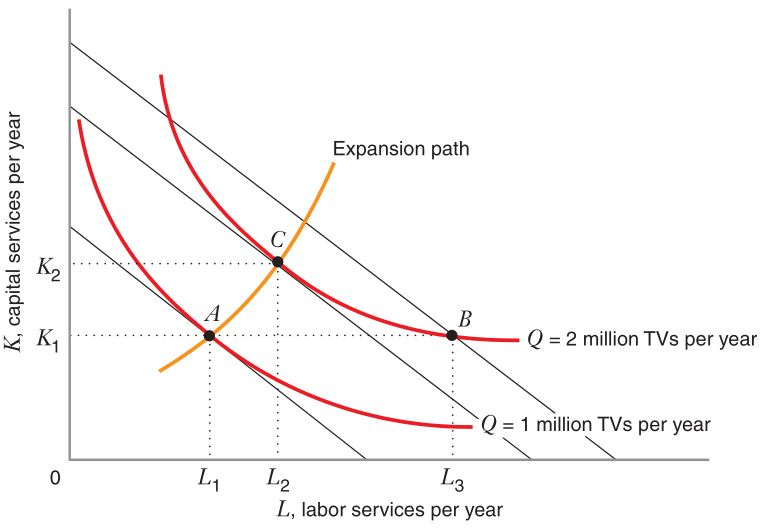
\includegraphics[width=220px]{figures/fig8_14.jpg}
  \end{figure}
\end{frame}

\begin{frame}{Relationship Between $LTC$ and $STC$}
  Note that total cost will \textbf{never} be lower in the short run than in the long run.

  \begin{itemize}
    \item If you can use that input combination in the short-run, you can use it in the long run!
  \end{itemize}
\end{frame}

\begin{frame}{Relationship Between $LTC$ and $STC$}
  Below are the STC and LTC curves for some firm. the $STC(Q)$ always lies above the $LTC(Q)$.
  \begin{figure}
    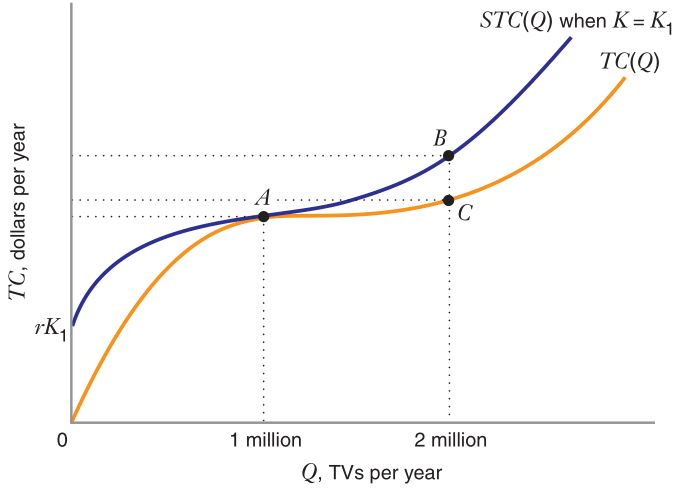
\includegraphics[width=220px]{figures/fig8_15.jpg}
  \end{figure}
\end{frame}

\begin{frame}{Short-Run Average and Marginal Cost Curves}
  We can define \textbf{short-run average cost}, $SAC$, and \textbf{short-run marginal cost}, $SMC$, similarly to their long-run counterparts.

  $$
    SAC(Q) = \frac{STC(Q)}{Q} \text{ and } 
    SMC(Q) = \frac{\Delta STC}{\Delta Q}
  $$

  \pause\bigskip
  We can also break SAC(Q) into average variable costs and average fixed costs.

  $$SAC(Q) = AVC(Q) + AFC(Q)$$
\end{frame}

\begin{frame}{Short-Run Average and Marginal Cost Curves}
  If we plot these curves, we can see that $SAC$ is found by vertically summing the $AFC$ and $ATC$ curves.

  \begin{itemize}
    \item The $AFC$ curve slopes downward because fixed costs do not change as output increases. The fixed cost is spread over more and more units of output.
    
    \item Note that the marginal cost curve intersects the average variable and average total cost curves at their minima.
  \end{itemize}
\end{frame}

\begin{frame}{Short-Run Average and Marginal Cost Curves}
  \begin{figure}
    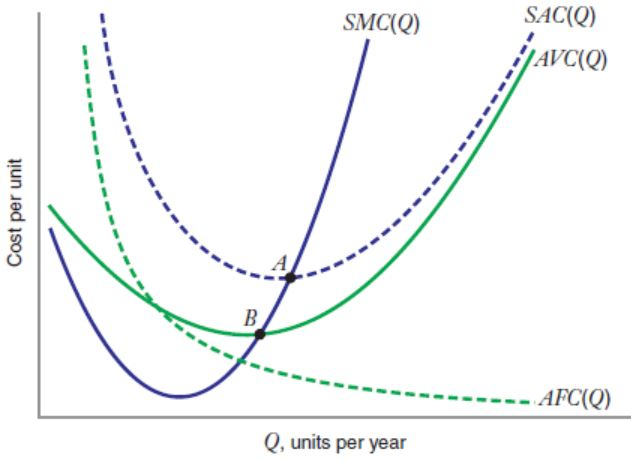
\includegraphics[width=240px]{figures/fig8_16.jpg}
  \end{figure}
\end{frame}

\begin{frame}{Relationship Between Long-Run and Short-Run $AC$ and $MC$ Curves}
  
  A firm can have many short-run average cost curves depending on the level of capital.

  \pause\bigskip
  In the long-run, capital can vary

  \begin{itemize}
    \item And the firm will choose the level of capital that minimizes average cost for a given output level.
    
    \item Thus, the long-run average cost curve is the boundary of all of the short-run average cost curves.
    
    \item It traces the minimum SAC for every level of output.
  \end{itemize}


\end{frame}

\begin{frame}
  The long-run curve can be thought of as the lower envelope of the set of short-run curves.
  \begin{figure}
    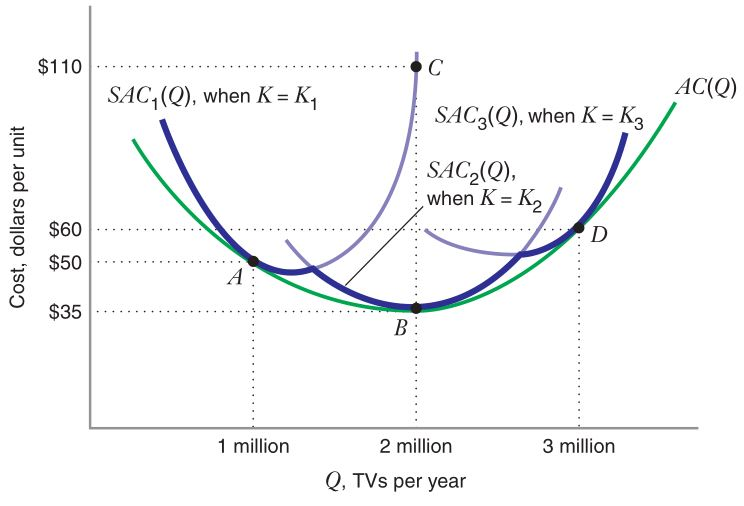
\includegraphics[width=280px]{figures/fig8_17.jpg}
  \end{figure}
\end{frame}

\begin{frame}
  \begin{figure}
    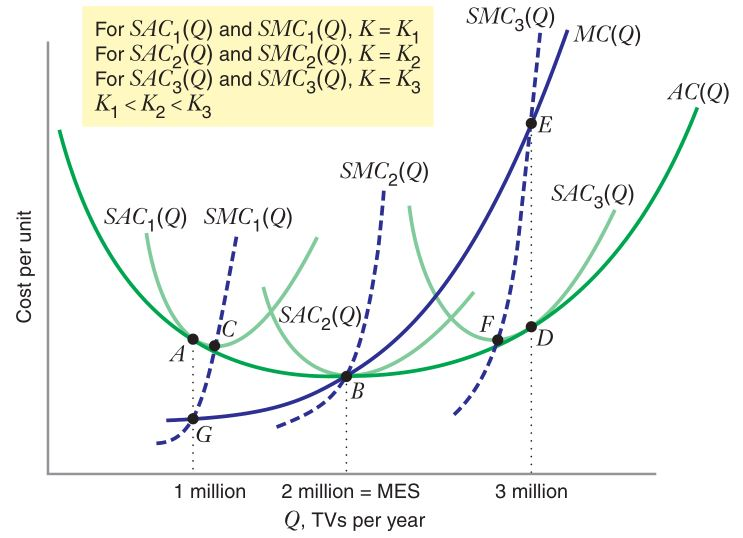
\includegraphics[width=280px]{figures/fig8_18.jpg}
  \end{figure}
\end{frame}

\begin{frame}{\bgCoral{Try It Yourself}}

\bigskip
Which of the following relationships is always true?
  \begin{enumerate}[A)]
    \item $MC(Q) > SMC(Q)$
    \item $AC(Q) > MC(Q)$
    \item $SAC(Q) > MC(Q)$
    \item $SAC(Q) > AC(Q)$
  \end{enumerate}
\end{frame}

\begin{frame}{Other Determinants of Cost}
  So far, we have focused on firms that only produce 1 good or service.

  \begin{itemize}
    \item But many firms sell a large variety of goods (Samsung, Johnson \& Johnson, General Electric).
  \end{itemize}

  \bigskip\pause
  Why do some firms choose to produce many different products?
  \begin{itemize}    
    \item Often, because fixed costs can be spread among many more units.
    
    \item For example, a satellite TV company broadcasts many channels... Not just one.
  \end{itemize}
\end{frame}

\begin{frame}{Other Determinants of Cost}
  Or Budweiser can use their machinery to bottle many different types of beer.

  \begin{itemize}
    \item Firms can also spread administrative costs over more units of output
    \begin{itemize}
      \item E.g. the accounting department or human resources department.
    \end{itemize}
  \end{itemize}

  Can also receive discounts on inputs (if their products use a common input) or shipping costs.
\end{frame}

\begin{frame}{Other Determinants of Cost}
  Mathematically, a firm is said to experience \textbf{economies of scope} if:

  $$
    TC(Q_1,Q_2) < TC(Q_1,0) + TC(0, Q_2)
  $$

  \bigskip
  In other words, the total cost of 1 firm producing both goods ($Q_1$ and $Q_2$) is less than the sum of the total costs of each firm producing separately

  \pause\bigskip
  The opposite could be true, implying \textbf{diseconomies of scope}
\end{frame}

\begin{frame}{Other Determinants of Cost}
  Sometimes costs can fall over time as a firm learns more efficient production methods.

  This is known as \textbf{economies of experience} or \textbf{learning-by-doing}.

  \pause\bigskip
  Think of the solar industry.
  \begin{itemize}
    \item The price of solar power has fallen 60\% in the last decade.
 
    \item This is at least partly a result of accumulated experience.
  \end{itemize}
\end{frame}

\end{document}
